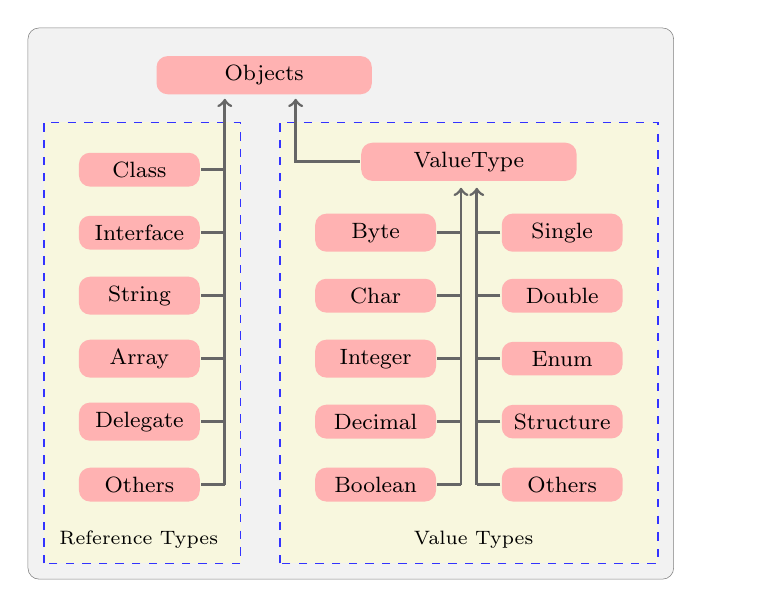
\begin{tikzpicture}[line width=1pt, draw=black!60]
\tikzstyle{every_node}=[font=\color{black}\footnotesize, text width=1.3cm, text centered, fill=red!30, rounded corners]
\tikzstyle{nnnn}=[anchor=center, text width=4cm, font=\color{black}\scriptsize]
\filldraw[fill=gray!10, draw=gray, line width=.2pt, rounded corners] (-.2cm,.8cm)  rectangle +(8.2cm, 7cm);

\filldraw[anchor=center] (2.8cm,7.2cm) node[style=every_node,text width=2.5cm] {Objects};

\filldraw[fill=yellow!20, fill opacity=.5, line width=.6pt,draw=blue!80, dashed] (0cm,1cm) rectangle +(2.5cm,5.6cm);
\filldraw[fill=yellow!20, fill opacity=.5, line width=.6pt,draw=blue!80, dashed] (3cm,1cm) rectangle +(4.8cm,5.6cm);
\filldraw (2.2cm, 1.3cm) node[style=nnnn] {Reference Types};
\filldraw (6.7cm, 1.3cm) node[style=nnnn] {Value Types};

\filldraw[anchor=center] (5.4cm,6.1cm) node[style=every_node,text width=2.5cm] (vt) {ValueType};
\draw[->] (vt) -| (3.2cm,6.9cm);

\foreach \a/\b in {2/Others,2.8/Delegate,3.6/Array,4.4/String,5.2/Interface,6/Class}
{\filldraw (2cm, \a cm) node[style=every_node,anchor=east] {\b};
  \draw (2cm, \a cm) -- (2.3cm, \a cm);}
\draw[->] (2.3cm,2cm) -- (2.3cm,6.9cm);
\foreach \a/\b in {2/Boolean,2.8/Decimal,3.6/Integer,4.4/Char,5.2/Byte}
{\filldraw (5cm, \a cm) node[style=every_node,anchor=east] {\b};
  \draw (5cm, \a cm) -- (5.3cm, \a cm);}
\draw[->] (5.3cm,2cm) -- (5.3cm,5.77cm);
\foreach \a/\b in {2/Others,2.8/Structure,3.6/Enum,4.4/Double,5.2/Single}
{\filldraw (5.8cm, \a cm) node[style=every_node,anchor=west] {\b};
  \draw (5.8cm, \a cm) -- (5.5cm, \a cm);}
\draw[->] (5.5cm,2cm) -- (5.5cm,5.77cm);
\end{tikzpicture}
